\clearpage

\section{Vista de Procesos}

La planificación de las consultas se diseñó con el objetivo de reducir el volumen de datos lo antes posible. Para ello, se aplican en primer lugar las proyecciones, eliminando las columnas irrelevantes, y los selects, descartando las filas que no cumplen los criterios de filtrado. Este enfoque no solo optimiza la ejecución al minimizar la cantidad de datos procesados en las etapas posteriores, sino que además reduce la complejidad de operaciones más costosas como group by y join.

\begin{figure}[H]
    \centering
    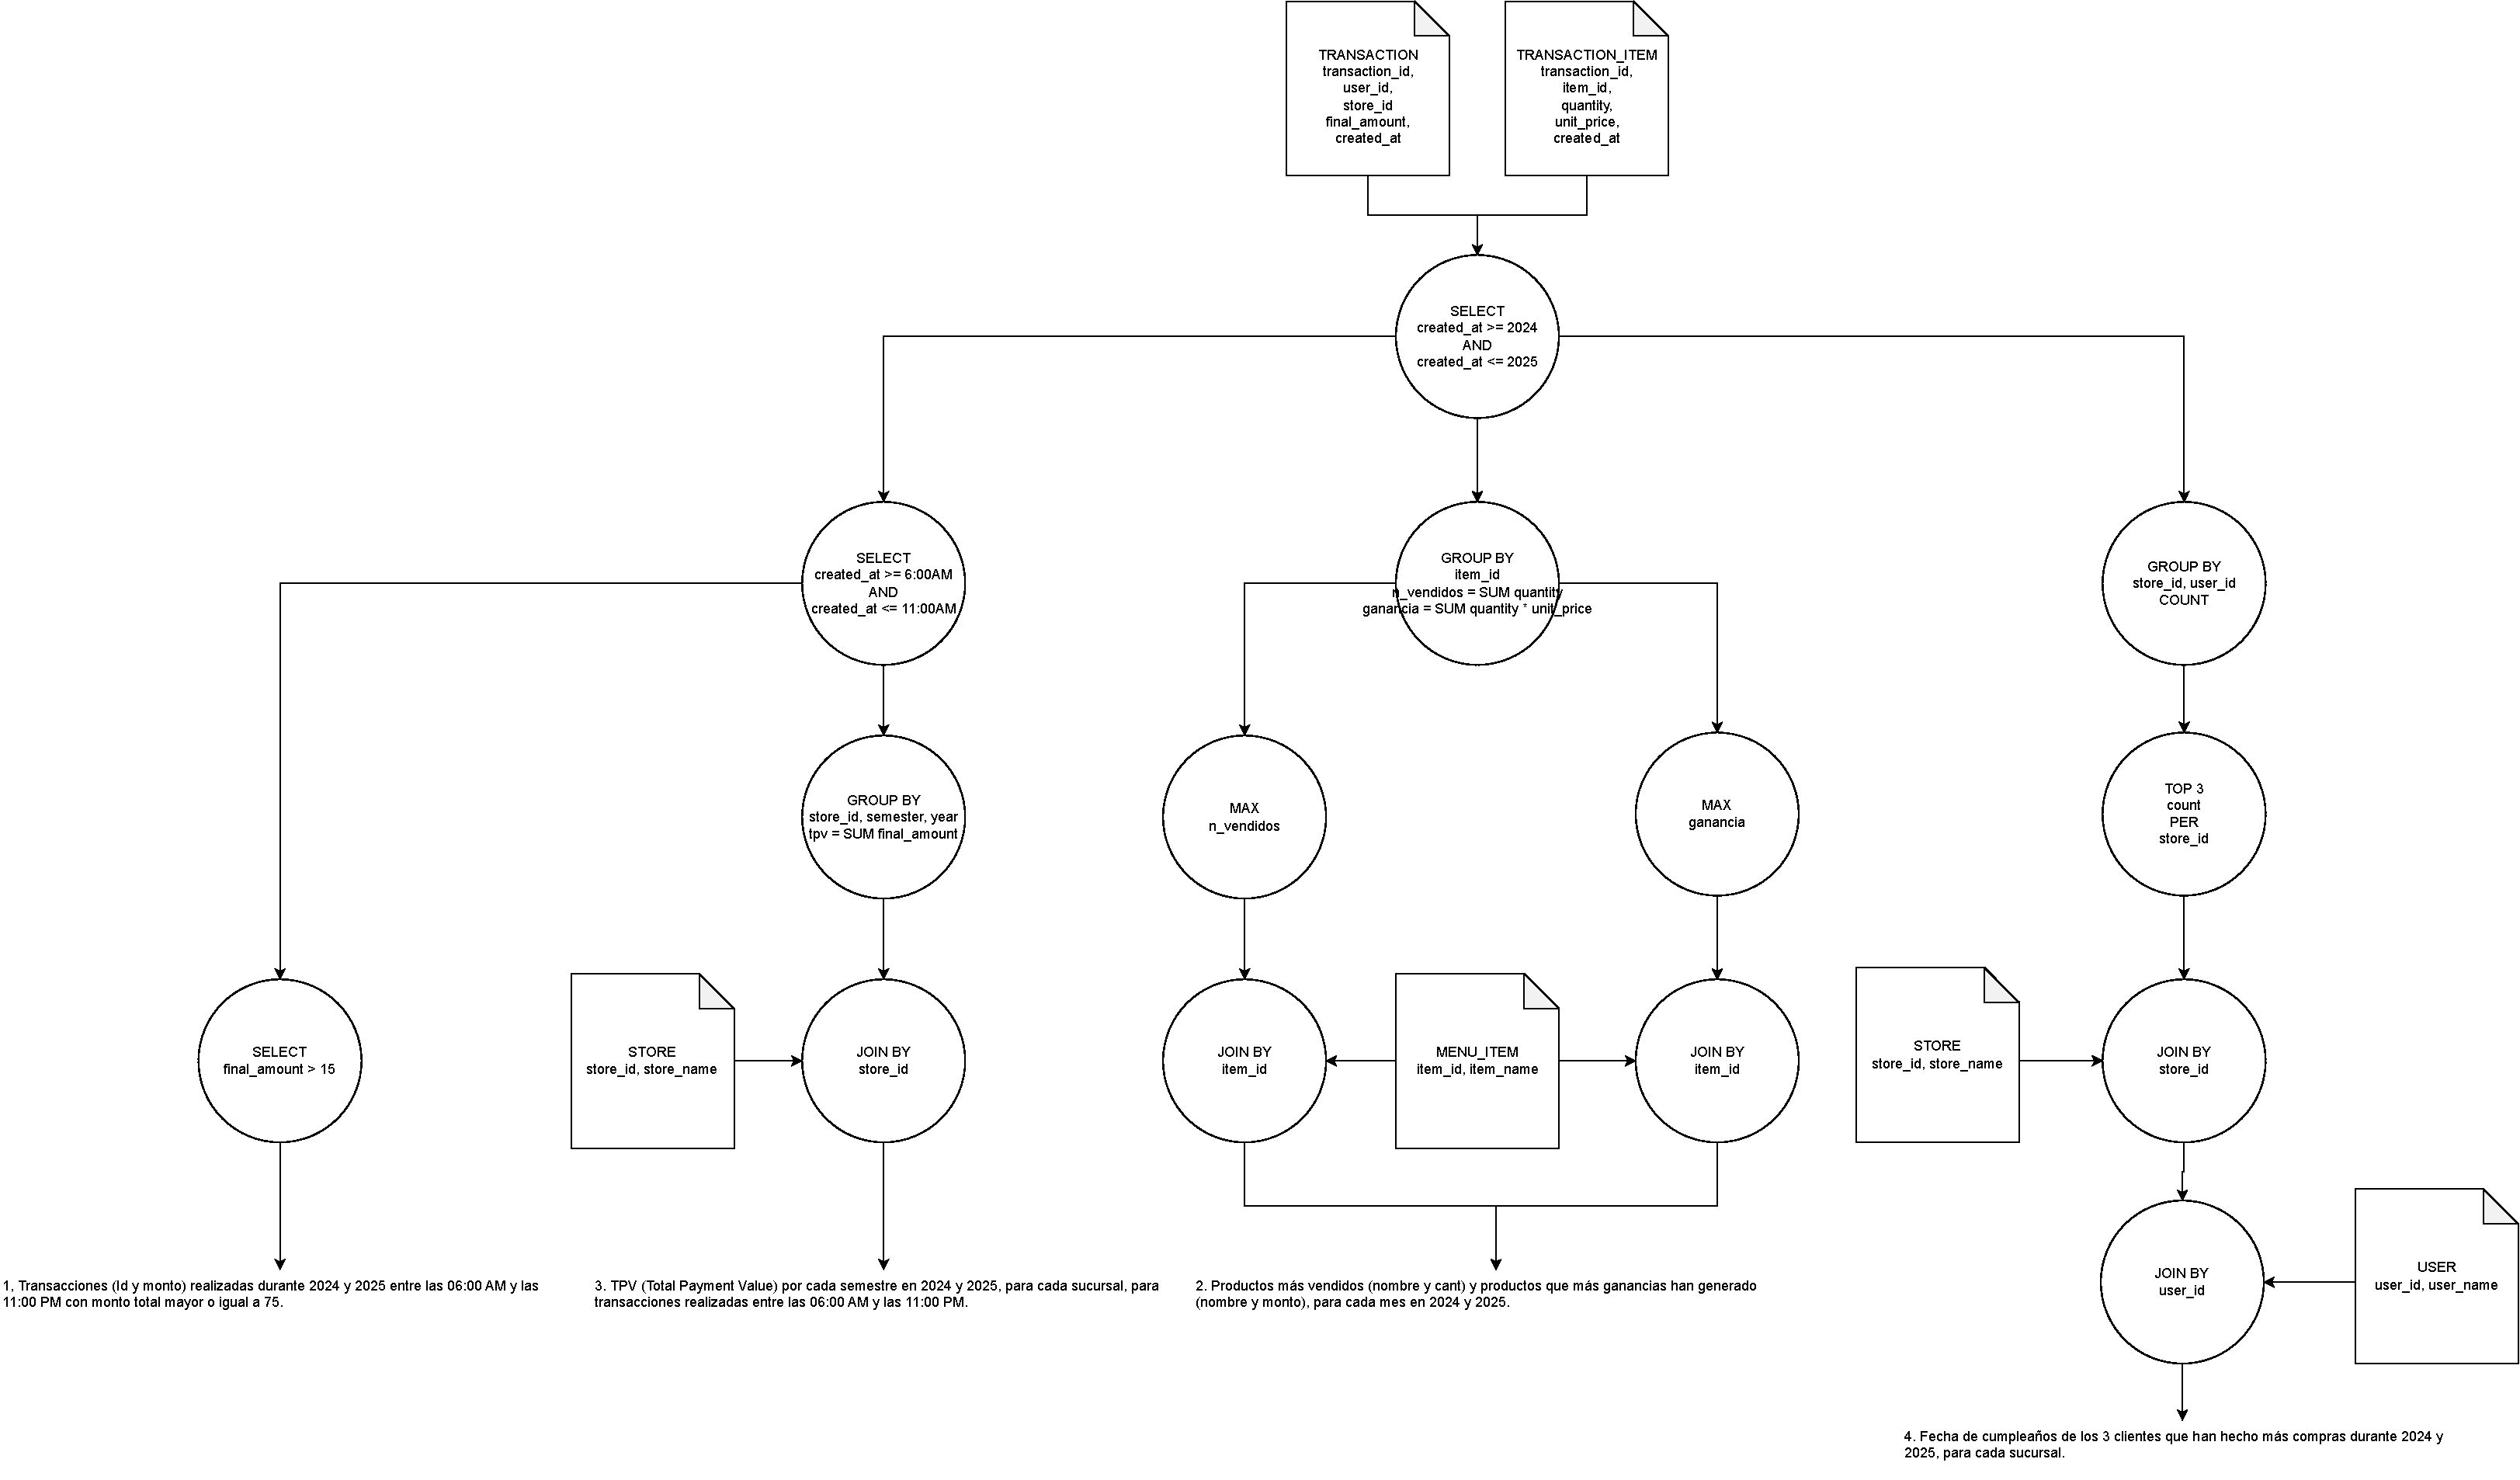
\includegraphics[width=1\textwidth]{img/vista_de_procesos/DAG.pdf}
    \caption{Diagrama DAG: Planificación de consultas}
\end{figure}

Ciertas tareas se pueden realizar en paralelo, por ejemplo la selección puede dividirse entre varios nodos ya que no es una operación que requiere de la totalidad de los datos para resolverse, a continuación se muestra como dos nodos de selección trabajan en paralelo.

\begin{figure}[H]
    \centering
    
\includegraphics[width=1\textwidth]{img/vista_de_procesos/actividades.pdf}
    \caption{Diagrama de actividades: Selección paralela}
\end{figure}

Este diagrama describe cómo un Select Node procesa las tareas que recibe a través del middleware.

El SelectNode consume las tareas desde la cola correspondiente utilizando consume\_select\_tasks. Cada tarea es derivada a un TypeHandler, que se obtiene con get\_handler(task.type\_query). El handler ejecuta la operación (exec(task.data)), produciendo un resultado parcial (task\_output). El resultado se envía al Middleware mediante send\_output, que utiliza un esquema de hashing (hash(key)) para determinar a qué GroupQueue debe ir. Finalmente, el GroupNode correspondiente recibe la tarea y ejecuta handle\_group(task), continuando con la siguiente etapa del pipeline.

\begin{figure}[H]
    \centering
    
\includegraphics[width=1\textwidth]{img/vista_de_procesos/select_node.pdf}
    \caption{Diagrama de secuencia: Select Node}
\end{figure}

Este diagrama describe cómo un Group Node procesa las tareas que recibe a través del middleware.

El GroupNode recibe tareas desde el middleware (handle(task)). Se obtiene el handler correspondiente mediante get\_handler(task.type\_query). El handler ejecuta la lógica de agrupación (exec(task.data)), generando resultados junto con una clave de partición (task\_output, hash\_key). El resultado se envía al middleware con send\_output, que utiliza hash(hash\_key) para decidir a qué JoinQueue corresponde. El JoinNode recibe los resultados parciales y continúa con las uniones necesarias.

\begin{figure}[H]
    \centering
    
\includegraphics[width=1\textwidth]{img/vista_de_procesos/groupby_node.pdf}
    \caption{Diagrama de secuencia: Group Node}
\end{figure}

\subsection{State Storage}

Los diferentes elementos que componen el sistema podrían verse afectados por un fallo en cualquier momento de su operación, por lo que podrían quedar ellos mismo o todo el sistema en un estado inconsistente.

En el siguiente diagrama se muestra como se utiliza el \textbf{State Storage} para asegurar la resiliencia a fallos y la consistencia de los datos ya procesados por el \textbf{Groupby Node}.

\begin{figure}[H]
    \centering
    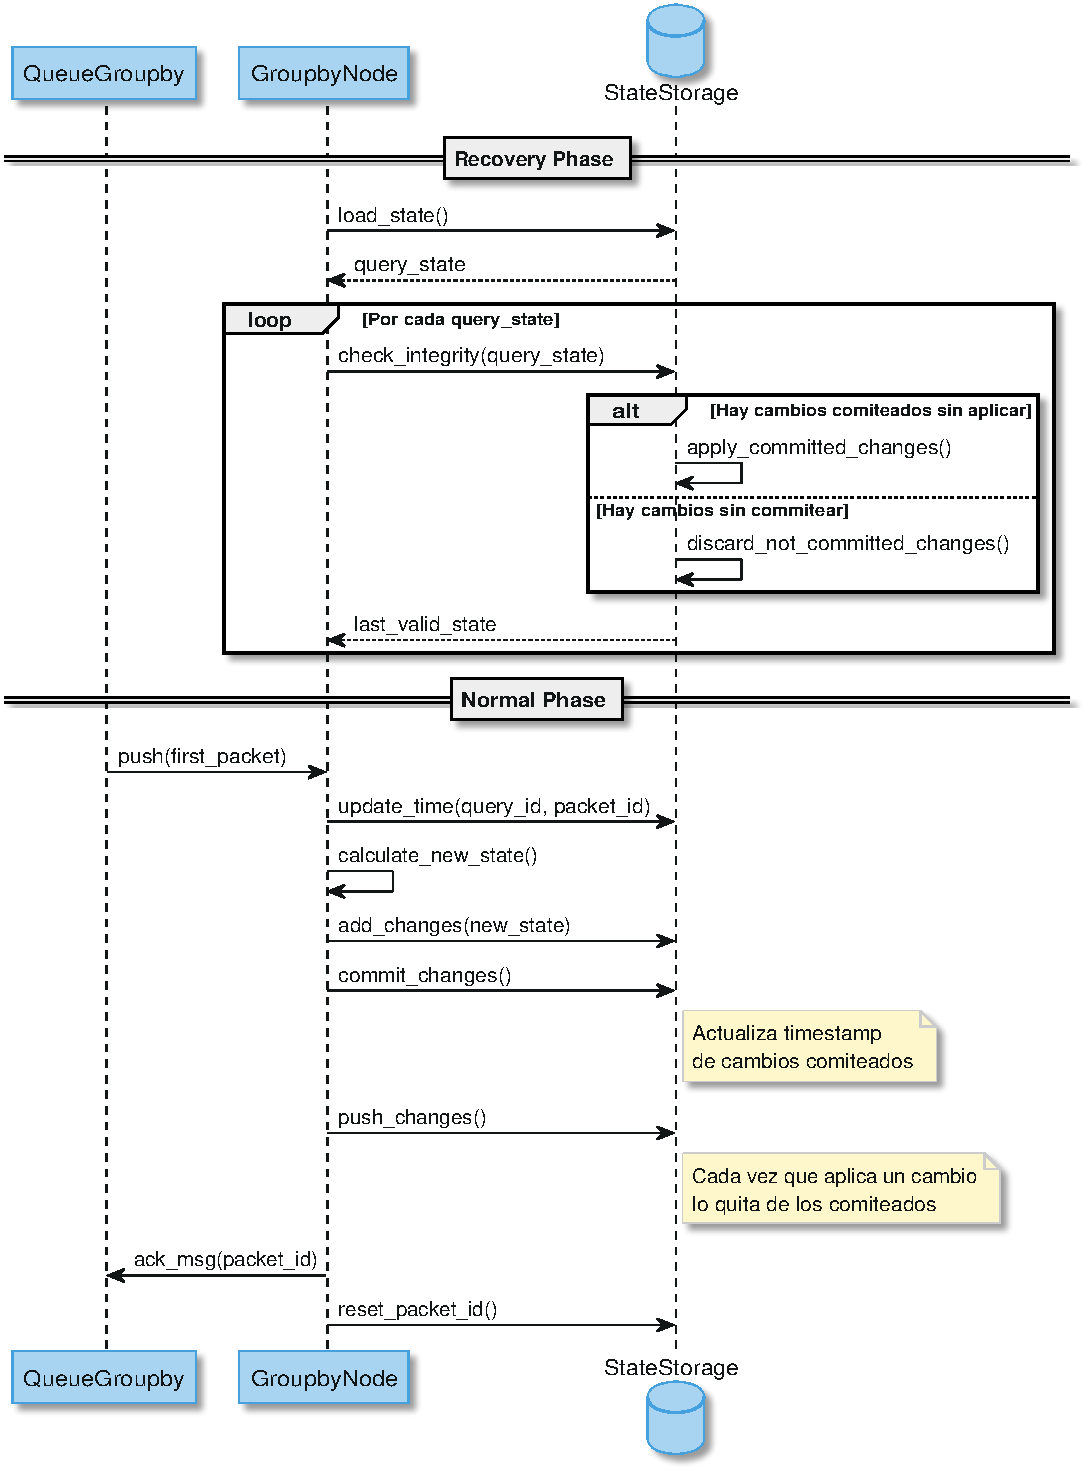
\includegraphics[width=1\textwidth]{img/vista_de_procesos/state_storage.pdf}
    \caption{Diagrama de secuencia: Interacción entre Groupby Node y su State Storage}
\end{figure}

\clearpage

\subsection*{Fase de Recuperación}

\begin{itemize}
  \item \textbf{Carga del Estado}: Se recupera el estado persistido que incluye:
    \begin{itemize}
      \item Estado actual de las queries
      \item Timestamp del último cambio aplicado
      \item Timestamp del último cambio comprometido
      \item ID del paquete en proceso
      \item Metadatos y tags adicionales
    \end{itemize}

  \item \textbf{Verificación de Integridad}: Para cada query almacenada:
    \begin{itemize}
      \item Si hay cambios comprometidos pendientes $\rightarrow$ Se aplican automáticamente
      \item Si hay cambios sin comprometer $\rightarrow$ Se descartan para mantener consistencia
      \item Se retorna el último estado válido
    \end{itemize}
\end{itemize}


\subsection*{Fase de Procesamiento Normal}

\begin{itemize}
  \item \textbf{Registro del Nuevo Paquete}:
    \begin{itemize}
      \item Se actualiza el timestamp del cambio actual
      \item Se almacena la información del paquete (query\_id, packet\_id, metadatos)
    \end{itemize}

  \item \textbf{Cálculo del Nuevo Estado}:
    \begin{itemize}
      \item Se procesa la lógica de negocio con los datos del paquete
      \item Se genera la nueva versión/cambios a aplicar
    \end{itemize}

  \item \textbf{Preparación de Cambios}:
    \begin{itemize}
      \item Se escriben los cambios en la sección temporal de cambios pendientes
    \end{itemize}

  \item \textbf{Compromiso de Cambios (commit\_changes)}:
    \begin{itemize}
      \item Se incrementa el timestamp de cambios comprometidos
      \item Los cambios pasan de ``pendientes'' a ``comprometidos'' (atomicidad)
    \end{itemize}

  \item \textbf{Aplicación de Cambios (push\_changes)}:
    \begin{itemize}
      \item Se fusionan los cambios comprometidos con el estado actual
      \item Se eliminan los cambios ya aplicados de la cola de comprometidos
    \end{itemize}

  \item \textbf{Finalización del Procesamiento}:
    \begin{itemize}
      \item Se envía ACK al mensaje para confirmar procesamiento exitoso
      \item Se limpia la información del paquete actual (reset\_packet\_id)
    \end{itemize}
\end{itemize}


Notese que, si bien el ejemplo utiliza el caso particular del \textbf{Groupby Node}, la lógica del \textbf{State Storage} no está acoplada a un estado específico.
En su lugar, emplea una interfaz de estado que define los mecanismos de serialización y deserialización.

Esto permite que el \textbf{State Storage} sea utilizado por distintos componentes del sistema, cada uno declarando el estado que necesita persistir según la función que desempeña.


\subsection{Eleccion de Lider: Bully}

El algoritmo Bully asegura que el supervisor con mayor identificador actúe como líder del sistema. La siguiente secuencia ilustra el caso donde \textbf{Supervisor2} (ID=2) se reintegra mientras \textbf{Supervisor1} (ID=1) está funcionando como líder, y cómo se realiza la transición de liderazgo sin perder monitoreo ni estado.

\begin{figure}[H]
    \centering
    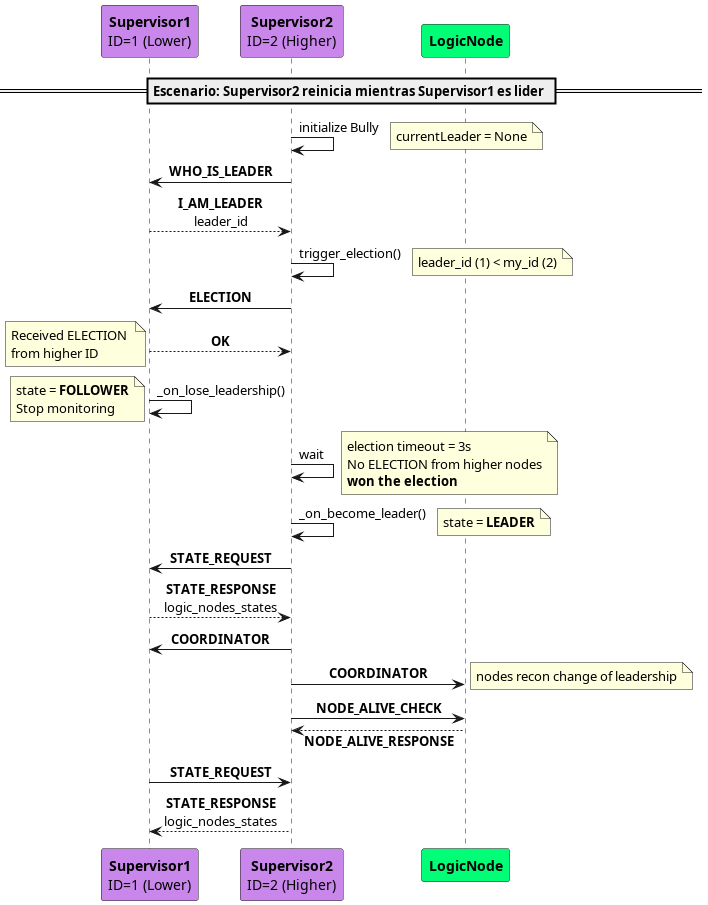
\includegraphics[width=1\textwidth]{img/vista_de_procesos/diagrama_eleccion_lider.png}
    \caption{Diagrama de secuencia: Ingresa un Supervisor de mayor ID que el lider}
\end{figure}

Hay dos supervisores:
\begin{itemize}
    \item \textbf{Supervisor1}: ID = 1 (prioridad menor), inicialmente líder.
    \item \textbf{Supervisor2}: ID = 2 (prioridad mayor), se reinicia y vuelve al cluster.
\end{itemize}

Al arrancar, Supervisor2 no asume nada y comienza en estado \texttt{FOLLOWER}.


Antes de disparar una elección, Supervisor2 pregunta quién es el líder:
\begin{itemize}
    \item Envía \texttt{WHO\_IS\_LEADER} a sus peers.
    \item Supervisor1 responde indicando que es el líder actual.
\end{itemize}

Con esa información, Supervisor2 compara IDs:
si el \texttt{leader\_id} recibido es menor que su propio ID, decide desafiar al líder y dispara el algoritmo Bully; si fuera mayor o igual, simplemente acepta al líder existente.


Cuando Supervisor2 decide desafiar:
\begin{itemize}
    \item Inicia una elección (\texttt{trigger\_election()}), enviando \texttt{ELECTION} a supervisores con ID mayor (en este caso no hay).
    \item Supervisor1, al recibir \texttt{ELECTION} desde un ID mayor, responde y deja de ser líder (pasa a \texttt{FOLLOWER} y desactiva su monitoreo).
    \item Tras un timeout sin respuestas de IDs mayores, Supervisor2 se proclama líder.
\end{itemize}


Al convertirse en líder, Supervisor2:
\begin{itemize}
    \item Cambia su estado a \texttt{LEADER} y activa el monitoreo de nodos.
    \item Recupera el estado de los nodos, ya sea desde el líder anterior o usando el estado replicado.
    \item Marca los nodos heredados como candidatos a checkear (pasando temporalmente a \texttt{SUSPECT}) y les envía checks activos para confirmar que siguen vivos.
\end{itemize}

De esta forma se evita asumir ciegamente un estado desactualizado y se revalida rápidamente qué nodos están realmente operativos.


Finalmente, el nuevo líder:
\begin{itemize}
    \item Anuncia su liderazgo mediante mensajes de \texttt{COORDINATOR} a otros supervisores.
    \item Continúa replicando periódicamente el estado para que un futuro cambio de líder pueda reutilizar esa información.
\end{itemize}


Este protocolo garantiza que:
\begin{itemize}
    \item Nunca haya dos líderes simultáneos (el líder anterior se desactiva antes de que el nuevo comience a monitorear).
    \item El líder con mayor ID sea quien coordina, siempre que esté disponible.
    \item Un supervisor que se reinicia pueda integrarse sin romper el servicio, desafiando al líder actual sólo cuando corresponde.
    \item La transición de liderazgo preserve el estado de los nodos y lo revalide rápidamente, manteniendo la funcionalidad de monitoreo y recuperación ante fallos.
\end{itemize}


En la siguiente secuencia quisimos detallar qué ocurre cuando el \textit{supervisor líder} se cae y cómo el sistema recupera automáticamente un nuevo líder usando el algoritmo Bully.


\begin{figure}[H]
    \centering
    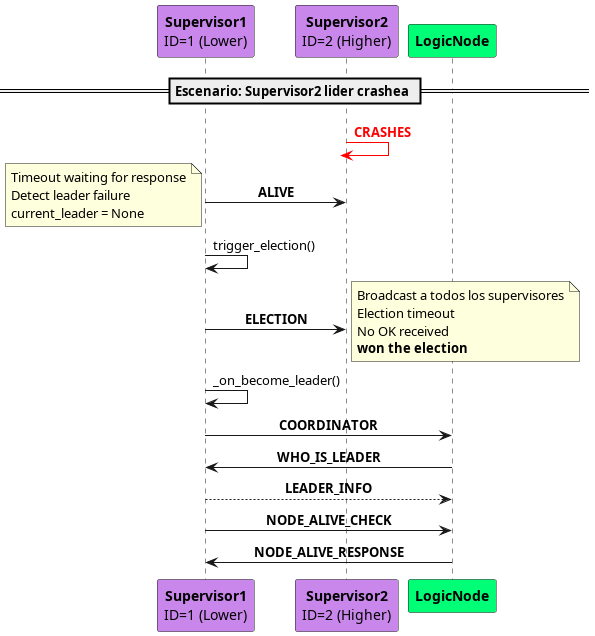
\includegraphics[width=1\textwidth]{img/vista_de_procesos/diagrama_eleccion_lider_crashea.png}
    \caption{Diagrama de secuencia: Cambio de lider por caida}
\end{figure}


En el estado inicial hay:
\begin{itemize}
    \item Un \textbf{supervisor líder} (ID más alto) que monitorea los nodos.
    \item Un \textbf{supervisor followers} que conoce quién es el líder actual.
    \item \textbf{LogicNodes} que envían heartbeats al líder.
\end{itemize}


El follower ejecuta un bucle de monitoreo del líder. Periódicamente verifica si sigue recibiendo señales de vida del líder (mensajes \texttt{ALIVE} o equivalente).  
Si durante un intervalo configurado no llega ninguna señal, el follower asume que el líder ha fallado y limpia \texttt{current\_leader}.



Al detectar el fallo, el follower dispara \texttt{trigger\_election()}:
\begin{itemize}
    \item Envía mensajes \texttt{ELECTION} a todos los supervisores con ID mayor.
    \item Si alguno responde, ese supervisor de mayor ID continuará la elección y eventualmente se proclamará líder.
    \item Si nadie responde (todos los IDs mayores están caídos), el follower gana por defecto.
\end{itemize}

Tras un \texttt{election\_timeout} sin respuestas de IDs mayores, el supervisor que inició la elección se convierte en nuevo líder.


Cuando un supervisor se proclama líder:
\begin{itemize}
    \item Cambia su estado interno a \texttt{LEADER} y actualiza \texttt{current\_leader}.
    \item Ejecuta un callback en \texttt{Supervisor} (\texttt{on\_become\_leader()}) para activar el monitoreo de nodos.
    \item A partir de este momento, comienza a enviar mensajes de \texttt{ALIVE} a los demás supervisores para que sepan quién es el líder actual.
\end{itemize}



Los LogicNode siguen enviando heartbeats al líder anterior hasta que dejan de recibir respuestas. Cuando detectan que el líder no responde:
\begin{itemize}
    \item Ejecutan un proceso de descubrimiento (\texttt{\_discover\_leader()}).
    \item Envían \texttt{WHO\_IS\_LEADER} a los supervisores.
    \item El nuevo líder responde con \texttt{LEADER\_INFO}, indicando su identidad y dirección.
    \item Los Nodos actualizan su \texttt{current\_leader} y redirigen los siguientes heartbeats al nuevo líder.
\end{itemize}


El diagrama de secuencia muestra cómo:
\begin{enumerate}
    \item El fallo del líder se detecta automáticamente por timeout.
    \item El algoritmo Bully elige un nuevo líder.
    \item Los Nodos redescubren al líder y retoman el envío de heartbeats.
\end{enumerate}

De esta forma, el sistema mantiene la funcionalidad de monitoreo y tolerancia a fallos incluso ante la caída completa del supervisor líder.

\subsection{Protocolo de comunicacion entre Healthchecker y Supervisor}

\begin{figure}[H]
    \centering
    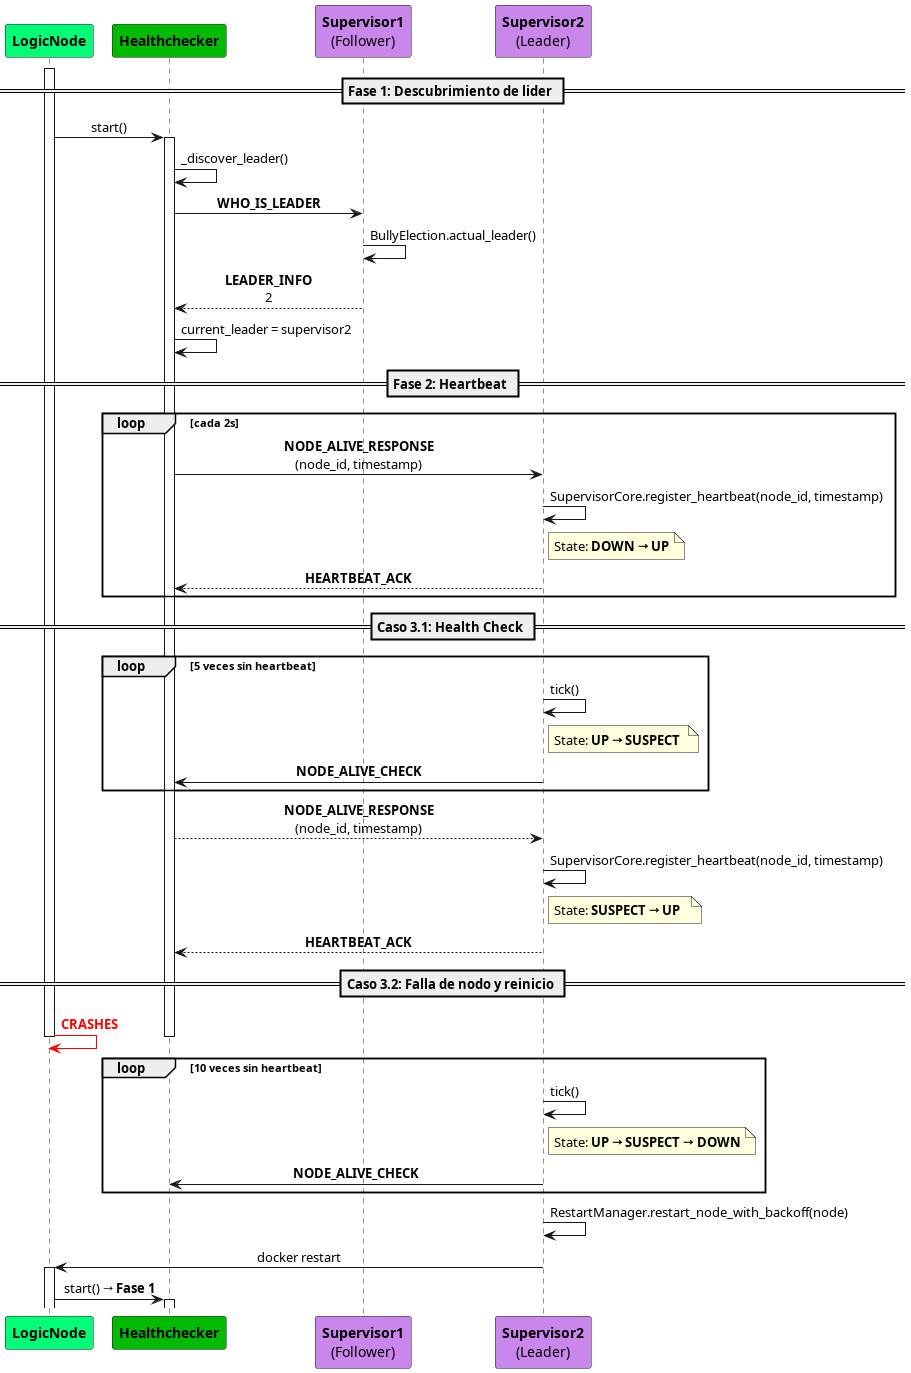
\includegraphics[width=0.9\textwidth]{img/vista_de_procesos/diagrama_secuencia_protocolos.png}
    \caption{Diagrama de secuencia: Protocolo de Healthchecker y Supervisor}
\end{figure}

El anterior diagrama describe cómo el \textbf{Healthchecker} de cada nodo se comunica con el \textbf{Supervisor líder} para monitorear disponibilidad y recuperar fallos.

Cuando un nodo inicia, no sabe quién es el líder. El Healthchecker envía \texttt{WHO\_IS\_LEADER} y un supervisor responde \texttt{LEADER\_INFO}. Esto permite:
\begin{itemize}
    \item Redirigir heartbeats al supervisor correcto.
    \item Evitar elecciones innecesarias.
\end{itemize}


Una vez que conoce al líder, el Healthchecker envía periódicamente \texttt{NODE\_ALIVE\_RESPONSE}.  
El líder:
\begin{itemize}
    \item Registra la actividad del nodo y lo marca \texttt{UP}.
    \item Responde con \texttt{HEARTBEAT\_ACK}.
\end{itemize}


Si el líder deja de recibir heartbeats por un período configurado, el nodo pasa a \texttt{SUSPECT}.  
Para descartar falsos positivos, el supervisor envía \texttt{NODE\_ALIVE\_CHECK}:
\begin{itemize}
    \item Si el worker responde, vuelve a \texttt{UP} sin reinicios.
    \item Se evita una recuperación innecesaria.
\end{itemize}


Si el nodo no responde dentro del umbral mas alto:
\begin{itemize}
    \item Se marca como \texttt{DOWN}.
    \item El \textbf{RestartManager} reinicia su contenedor.
    \item Cuando el nodo vuelve, repite la fase de \textbf{Descubrimiento de líder} y se reincorpora automáticamente.
\end{itemize}


Este protocolo combina:
\begin{itemize}
    \item Detección rápida de fallos reales.
    \item Protección ante falsos positivos.
    \item Recuperación automática.
\end{itemize}

Asegurando que el sistema mantenga siempre monitoreo activo y disponibilidad del servicio aún frente a fallos de nodos.
